\section{การวัดคลื่นไฟฟ้าบนร่างกาย}

อุปกรณ์วัดคลื่นไฟฟ้าบนร่างกายโดยส่วนมากมักเป็นอุปกรณ์ทางการแพทย์ (medical equipments) ซึ่งต้องมีความแม่นยำและ
ความถูกต้องสูง เนื่องจากความถูกต้องในการอ่านค่าเพื่อวินิจฉัยโรคเป็นสิ่งสำคัญ จะผิดพลาดไม่ได้

อย่างไรก็ดี กระแสของ "นักสร้าง" (makers) ในกลุ่มนักพัฒนาและผู้สนใจในเทคโนโลยี ทำให้การเข้าถึงอุปกรณ์ดังกล่าวเป็นไปได้ง่ายขึ้น
เนื่องด้วยมีความพยายามในการสร้างฮาร์ดแวร์เปิดซอร์ส (open-source hardware) สำหรับวัดคลื่นดังกล่าว

\subsection{โอเพนบีซีไอ (OpenBCI)}

(Todo: OpenBCI image)
 
โอเพ่นบีซีไอ (OpenBCI) เป็นฮาร์ดแวร์แบบเปิดซอร์ส (open-source harware) สำหรับการวัดค่าทางชีวภาพ (biosensing)
อันได้แก่ค่าศักย์ไฟฟ้าในร่างกายมนุษย์ ตัวฮาร์ดแวร์เปิดแบบผังออกมาในลักษณะเดียวกับที่อาร์ดูโน่ (Arduino)
เปิดผังการออกแบบวงจรเป็นสาธารณะ

โอเพ่นบีซีไอสามารถใช้ในการวัดค่าความต่างศักย์ไฟฟ้าซึ่งเกิดจากทั้งสมอง (EEG) กล้ามเนื้อ (EMG) และหัวใจ (EKG)
โดยตัวบอร์ดเป็นวงจรตรรกะแบบ 32 บิทซึ่งใช้ชิป ADS1229 สำหรับการวัดค่าไฟฟ้าร่างกาย ผลิตโดยบริษัท Texas Instruments
และรองรับการวัดช่องสัญญาณได้สูงสุด 8 ช่องสัญญาณพร้อมกัน

\subsection{อิเล็กโทรด (Electrode)}

\begin{figure}[h]
    \centering
    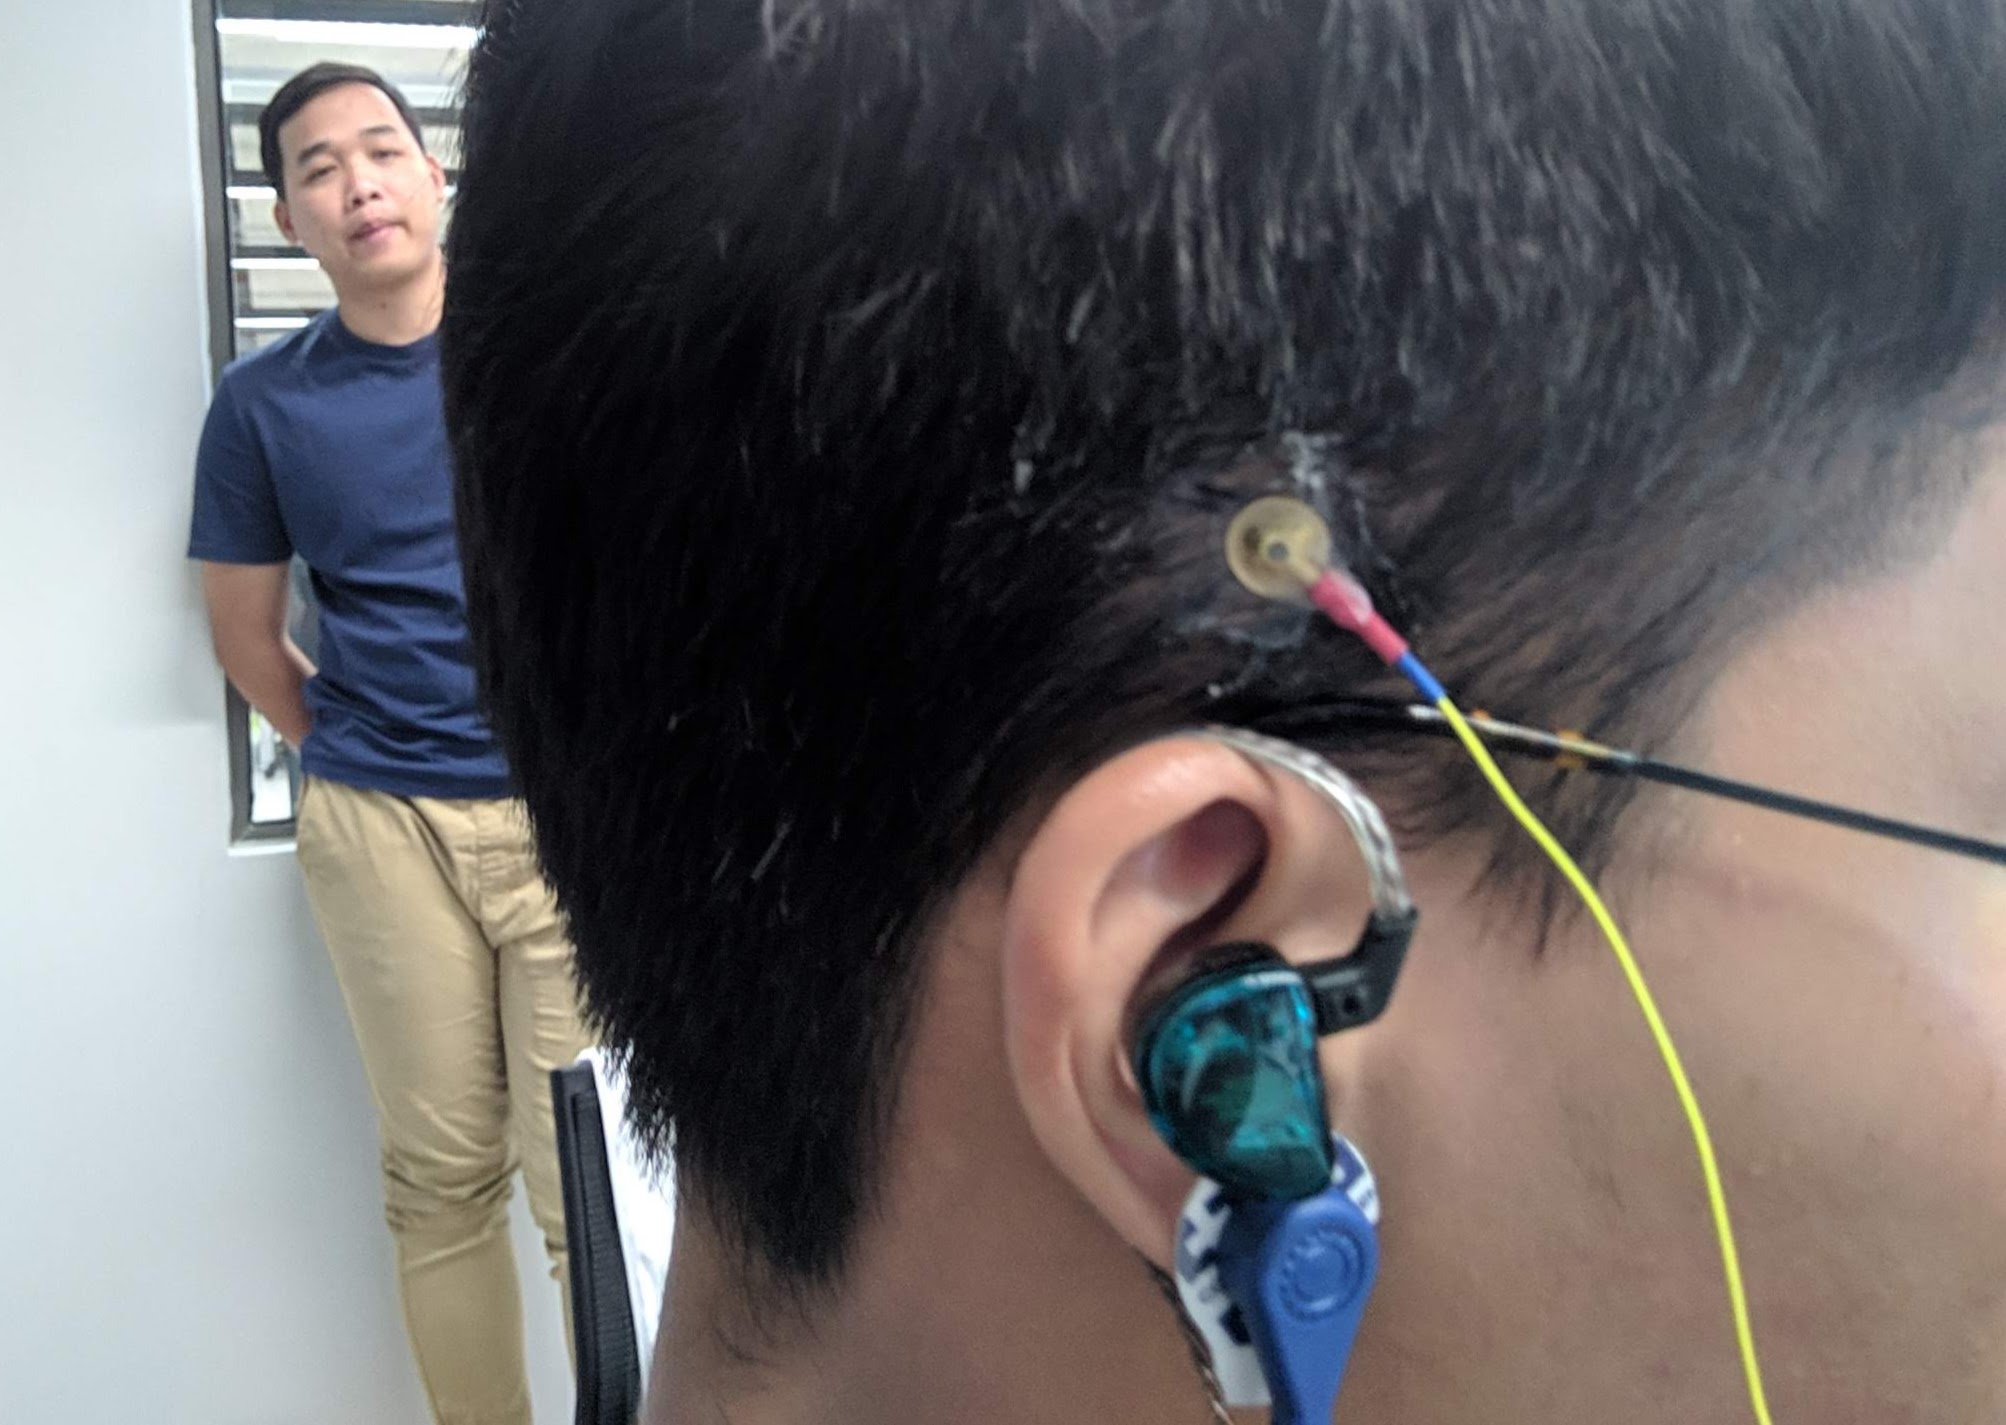
\includegraphics[width=0.5\textwidth]{images/IMG_20190610_155141.jpg}
    \caption{จากบนลงล่าง: อิเล็กโทรดแบบถ้วยทอง (Gold Cup) พร้อมสายสีเหลือง, หูฟัง, และอิเล็กโทรดแบบเจง (Gel) บริเวณติ่งหู}
\end{figure}

อิเล็กโทรดคือขั้วไฟฟ้าที่ทำการติดบนผิวหนังเพื่อวัดค่าศักย์ไฟฟ้าบริเวณจุดต่างๆ ที่สนใจ โดยมากมักใช้อิเล็กโทรดแบบ\textbf{ถ้วยทอง}
(Gold cup electrodes) และแบบ\textbf{เจล} (Get electrodes) ซึ่งสามารถเทียบกันได้ดังนี้

\begin{table}[H]
    \begin{tabularx}{\textwidth}{l|X|X}
         & แบบถ้วยทอง & แบบเจล\\
        \hhline{===}
        การทำความสะอาดผิวหนัง  & \multicolumn{2}{l}{ต้องทำความสะอาดผิวหนังก่อน}\\
        \hline
        การติดอิเล็กโทรด & ต้องใช้ยานำไฟฟ้าผิวหนัง (skin conducting paste) เสมอ  & อาจไม่ใช้ยานำไฟฟ้าผิวหนัง (skin conducting paste) แต่การใช้จะให้ผลลัพธ์ที่ดีกว่า \\
        \hline
        ความง่ายในการติด & ติดง่ายกว่าบริเวณที่มีผมหนา & ติดผิวหนังยากกว่าหากมีผมหนา\\
        \hline
        ความเปรอะเปื้อน & มาก เพราะยานำไฟฟ้าผิวหนังจะติดบริเวณผมและศีรษะ & น้อย เจลสามารถลอกออกได้จากผิวหนังโดยไม่ทิ้งคราบ\\
        \hline
        ราคา & ถูกกว่า ใช้ซ้ำได้ & แพงกว่า ส่วนเจลใช้ได้ครั้งเดียว\\
    \end{tabularx}
    \caption{ตารางเปรียบเทียบชนิดของอิเล็กโทรด}
\end{table}
